\clearpage

\section{Fermat’n kasino}

Vampyyri Fermat järjestää kartanossaan iltaisin uhkapeli-iltoja. Yksi pelaajista, kreivi Pascal, on kovasti tykästynyt rulettiin. Pascal uskoo, että pelaajat jäävät siinä keskimäärin voitolle.


Jokaisen peli-illan jälkeen Pascal lähtee kuitenkin tyhjin taskuin kotiin. 


Selittääkö epäonni Pascalin huonon menestyksen peli-illoissa?


Fermat’n rulettipöydässä yksi veikkaus maksaa 1 €.


\begin{figure}[h]
    \begin{center}
    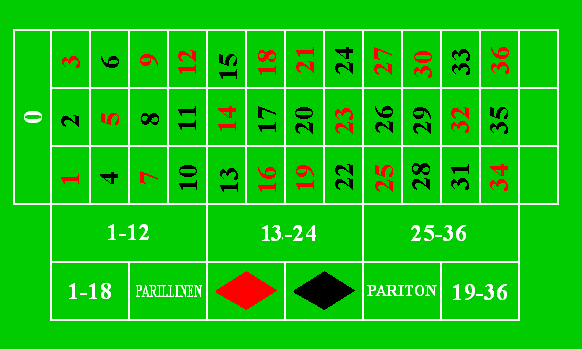
\includegraphics[width=0.8\linewidth]{kuvat/ruletti.png}
    \caption*{Rulettipöytä}
    \end{center}
\end{figure}

\begin{table}[h]
  \centering
    \begin{tabular}{| l | l | l |}
    \hline
    Panostusvaihtoehto & Selite & Voitto \\
    \hline
    Yksi numero & Pelimerkki sijoitettu yhdelle numerolle & 36 € \\
    Kaksi numeroa & Pelimerkki sijoitettu 2:n numeron rajalle & 18 € \\
    Neljä numeroa & Pelimerkki sijoitettu 4:n numeron kulmaan & 9 € \\
    \hline
    Tusinat & 1-12, 13-24 tai 25-36 & 3 € \\
    Väri & musta tai punainen & 2 € \\
    Pienet/isot & 1-18 tai 19-36 & 2 € \\
    Parillinen/pariton & & 2 € \\
    \hline
    \end{tabular}
  \caption*{Ruletin voitonjako}
\end{table}

Vihje: Mitä odotusarvo kertoo?